%% Hierarchical Taxonomic Abstraction for Safe Handling of Novel Objects
%% Paper v1 -- generated deliverable, compiles with pdflatex (IEEEtran).
\documentclass[conference]{IEEEtran}
\IEEEoverridecommandlockouts

\usepackage{graphicx}
\usepackage{amsmath,amssymb}
\usepackage{booktabs}
\usepackage{algorithm}
\usepackage{algorithmic}
\usepackage{xcolor}
\usepackage{url}
\usepackage[hidelinks]{hyperref}
\usepackage{orcidlink}

\graphicspath{{../figures/}{../images/}}

\newcommand{\floor}{$\blacklozenge$}

\begin{document}

\title{Hierarchical Taxonomic Abstraction for the Safe\\
Handling of Novel Objects in Autonomous Driving Perception}

\author{\IEEEauthorblockN{Felix Schaller \orcidlink{0000-0002-3218-3214}
\href{https://orcid.org/0000-0002-3218-3214}{0000-0002-3218-3214}}
\IEEEauthorblockA{Independent Researcher\\
Dubai, UAE / Munich, Germany\\
Email: \href{mailto:inquiry@felixschaller.com}{inquiry@felixschaller.com}}}

\maketitle

\begin{abstract}
Object detectors for autonomous driving classify against a \emph{flat} list of
categories. When a scene contains an object that does not fit any of those
categories---an overloaded rural truck, a horse trailer, a horse-drawn
carriage---a flat classifier must either force a confident but wrong label or
drop the object entirely. Both outcomes are unsafe. Building on a semantic-model
framework for constraining pattern recognition, we replace the flat list with a
\emph{hierarchical taxonomy} and add a runtime \emph{abstraction} mechanism:
detections descend the taxonomy only as far as the visual evidence justifies and
otherwise fall back to a coarser, still safety-relevant category. A per-branch
\emph{safety floor} bounds this fallback so the system never collapses into a
useless generic bucket; below the floor it emits an explicit, localized
\textsc{unknown obstacle}. Using pretrained YOLO boxes and CLIP zero-shot leaf
scoring (no training), we evaluate a fair head-to-head against a flat baseline on
the SegmentMeIfYouCan Road~Anomaly set. On novel objects the hierarchy handles
$100\%$ safely (abstracted or flagged) versus $0\%$ for the flat baseline, while
on known objects it remains at least as specific ($77\%$ vs.\ $47\%$ useful) and
never makes a confident wrong claim.
\end{abstract}

\begin{IEEEkeywords}
autonomous driving, object detection, semantic taxonomy, novelty handling,
open-set recognition, functional safety, CLIP.
\end{IEEEkeywords}

\section{Introduction}
\label{sec:intro}

Perception is the first link in the autonomous-driving stack, and its failures
propagate. Modern detectors are trained to recognize a fixed, one-dimensional
list of classes---\texttt{car}, \texttt{truck}, \texttt{person},
\texttt{bicycle}, and a handful more. This design is adequate on the curated
distributions of Western benchmarks but breaks in the open world, where the tail
of ``things on the road'' is effectively unbounded.

Figure~\ref{fig:title} illustrates the failure mode. In dense, improvised
traffic---common outside the datasets that detectors are tuned on---vehicles are
routinely loaded far beyond their canonical shape, mixed with animal-drawn carts
and hand-built conveyances. Such objects match \emph{no} flat category well. A
flat classifier then has only two moves, both unsafe: assign a confident label
that is wrong (misinforming downstream motion planning about size and behavior),
or, under a rejection threshold, discard the detection so that a real obstacle
silently disappears. This is the \emph{thesis}: the flat class list is itself a
safety hazard in the open world.

\begin{figure}[t]
\centering
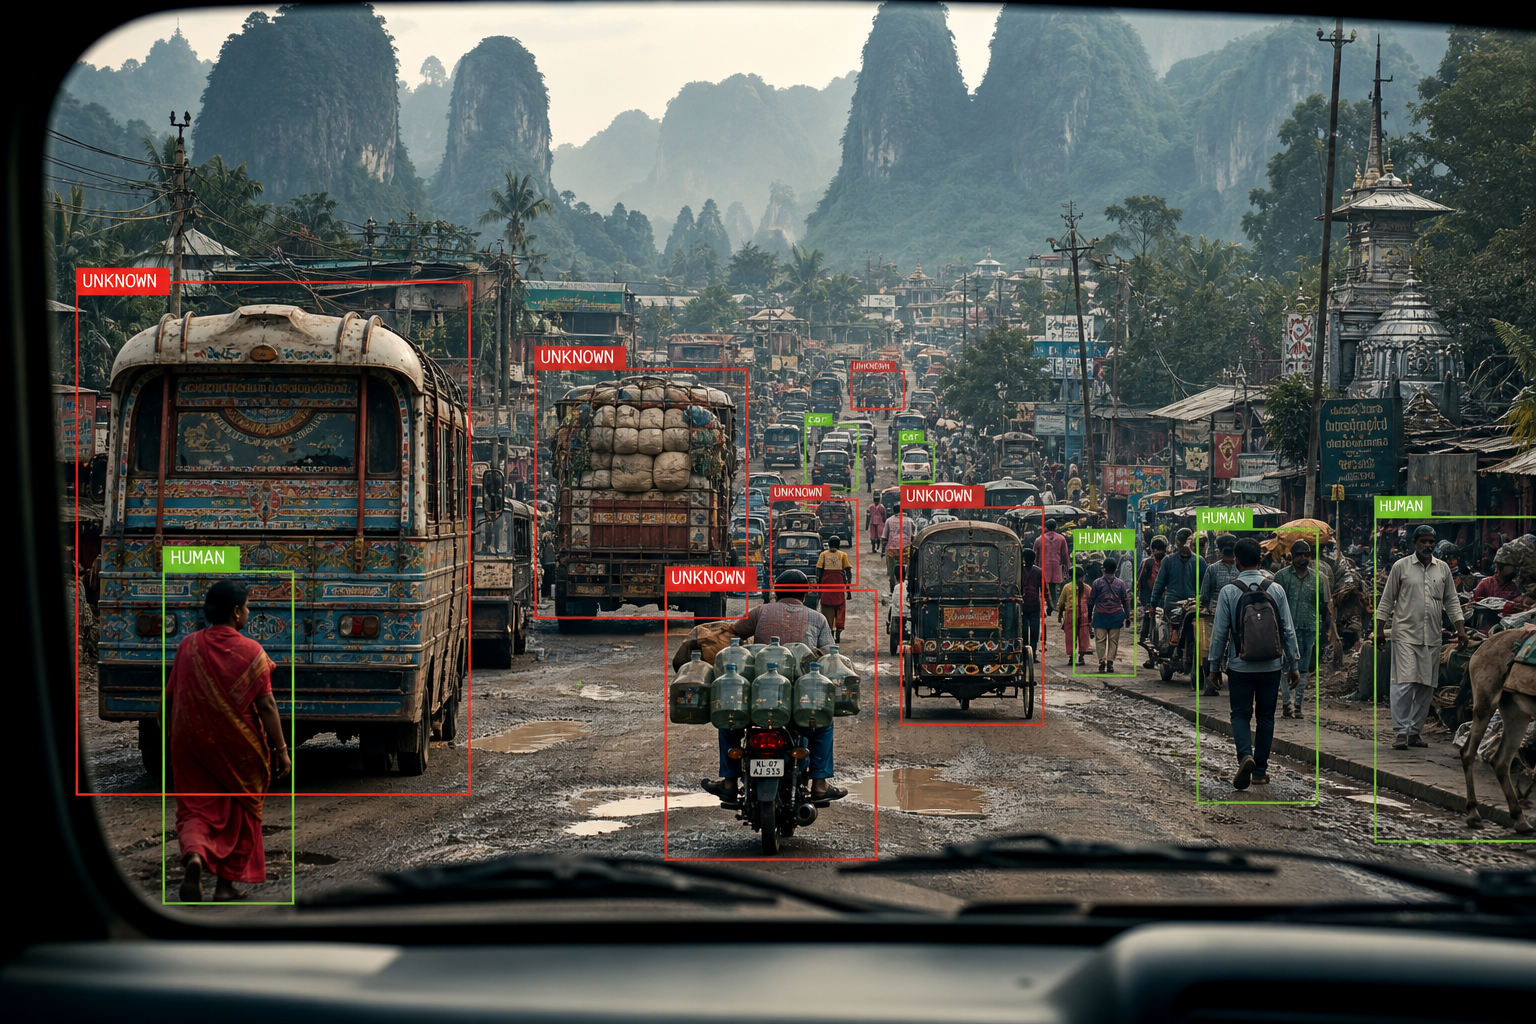
\includegraphics[width=\columnwidth]{YOLO-Traffic-Scene.png}
\caption{Motivating scenario (illustrative). In improvised, densely loaded
traffic many objects fit no canonical class. A flat detector must either
mislabel them or drop them; both are unsafe. Our system instead abstracts each
object up a taxonomy to the most specific level it can still justify, or flags an
explicit \textsc{unknown obstacle}.}
\label{fig:title}
\end{figure}

The remedy we pursue, following the semantic-model argument of
Schaller~\cite{schaller2025}, is to give perception a \emph{structured} label
space. This is the perception-level answer to the decidability crisis of
\cite{schaller_patterns}: because \emph{patterns are everywhere}, an ungrounded
inductive detector cannot decide whether a detected pattern is a physical truth
or an accidental correlation, so safety must be imposed \emph{structurally}, by
an over-arching, non-inductive meta-structure that governs classification at
runtime. Our taxonomy, with its safety floor, is exactly such a meta-structure.
Instead of a flat list, categories form a \emph{taxonomy}
(Fig.~\ref{fig:taxonomy}): \textsf{MAN~Truck} is a \textsf{Heavy~Truck} is a
\textsf{Truck} is a \textsf{Transport~Vehicle} is a \textsf{Vehicle}. When the
specific leaf cannot be identified, the system does not fall into the void---it
\emph{abstracts upward} until it reaches a category that is still confident and
useful. A horse trailer that is neither clearly a vehicle nor clearly an animal
is not forced into either; it is retained as a moving obstacle.

Abstraction alone, however, invites a second failure: the higher one climbs, the
more trivially true the label becomes. Reporting everything as ``an object'' is
correct and useless---a planner fed that label would brake for the entire world.
We therefore bound abstraction with a \emph{safety floor}: a per-branch limit
below which a label is still safety-actionable (\textsf{Vehicle},
\textsf{Living~Being}, \textsf{Static~Object}) and above which the system instead
emits a localized \textsc{unknown obstacle}. The floor is the anti-paranoia
counterpart to abstraction.

\textbf{Contributions.} (i) A runtime hierarchical-abstraction classifier that
scores only concrete taxonomy \emph{leaves} with a pretrained open-vocabulary
model and aggregates the resulting probability mass upward, descending only while
a single sub-branch dominates. (ii) A per-branch \emph{safety floor} that
converts over-abstraction into an explicit unknown rather than a useless generic
label. (iii) A fair, training-free head-to-head benchmark quantifying the safety
gain of the taxonomy over a flat list on real anomalous road scenes.

\section{Related Work}
\label{sec:related}

Class hierarchies have long been known to improve the \emph{quality} of
mistakes: Bertinetto et al.~\cite{bertinetto2020} show that hierarchy-aware
training makes wrong predictions less severe by keeping them semantically close.
We use the hierarchy at \emph{inference} time as an abstraction mechanism rather
than as a training loss. Open-vocabulary recognition via image--text embeddings,
established by CLIP~\cite{radford2021}, lets us score arbitrary taxonomy nodes
without task-specific training. Novelty and anomaly detection for driving is an
active area; autoencoder-based novelty detection~\cite{sedeh2021} flags
out-of-distribution inputs but, as noted in~\cite{schaller2025}, primarily at
training time and without a semantic interpretation. Benchmarks such as
SegmentMeIfYouCan~\cite{chan2021} and CODA~\cite{li2022} provide the anomalous
road objects on which such claims can be tested. Our method is complementary: it
provides an \emph{immediate, runtime} semantic fallback at a controllable level
of abstraction. The cognitive plausibility of graded, hierarchical categories is
long established in psychology~\cite{rosch1975}.

\section{Method}
\label{sec:method}

\subsection{Object Taxonomy}
The label space is a tree $T$ (Fig.~\ref{fig:taxonomy}) whose root is the generic
\textsf{Object} and whose leaves are concrete categories, a subset of which map
onto the detector's native (COCO) classes. Each node carries optional metadata:
a \emph{safety-floor} flag, a plausible size range, and a position prior. Three
nodes are floors: \textsf{Living~Being}, \textsf{Vehicle}, and
\textsf{Static~Object}---the coarsest trichotomy that still implies distinct
driving responses.

\begin{figure*}[t]
\centering
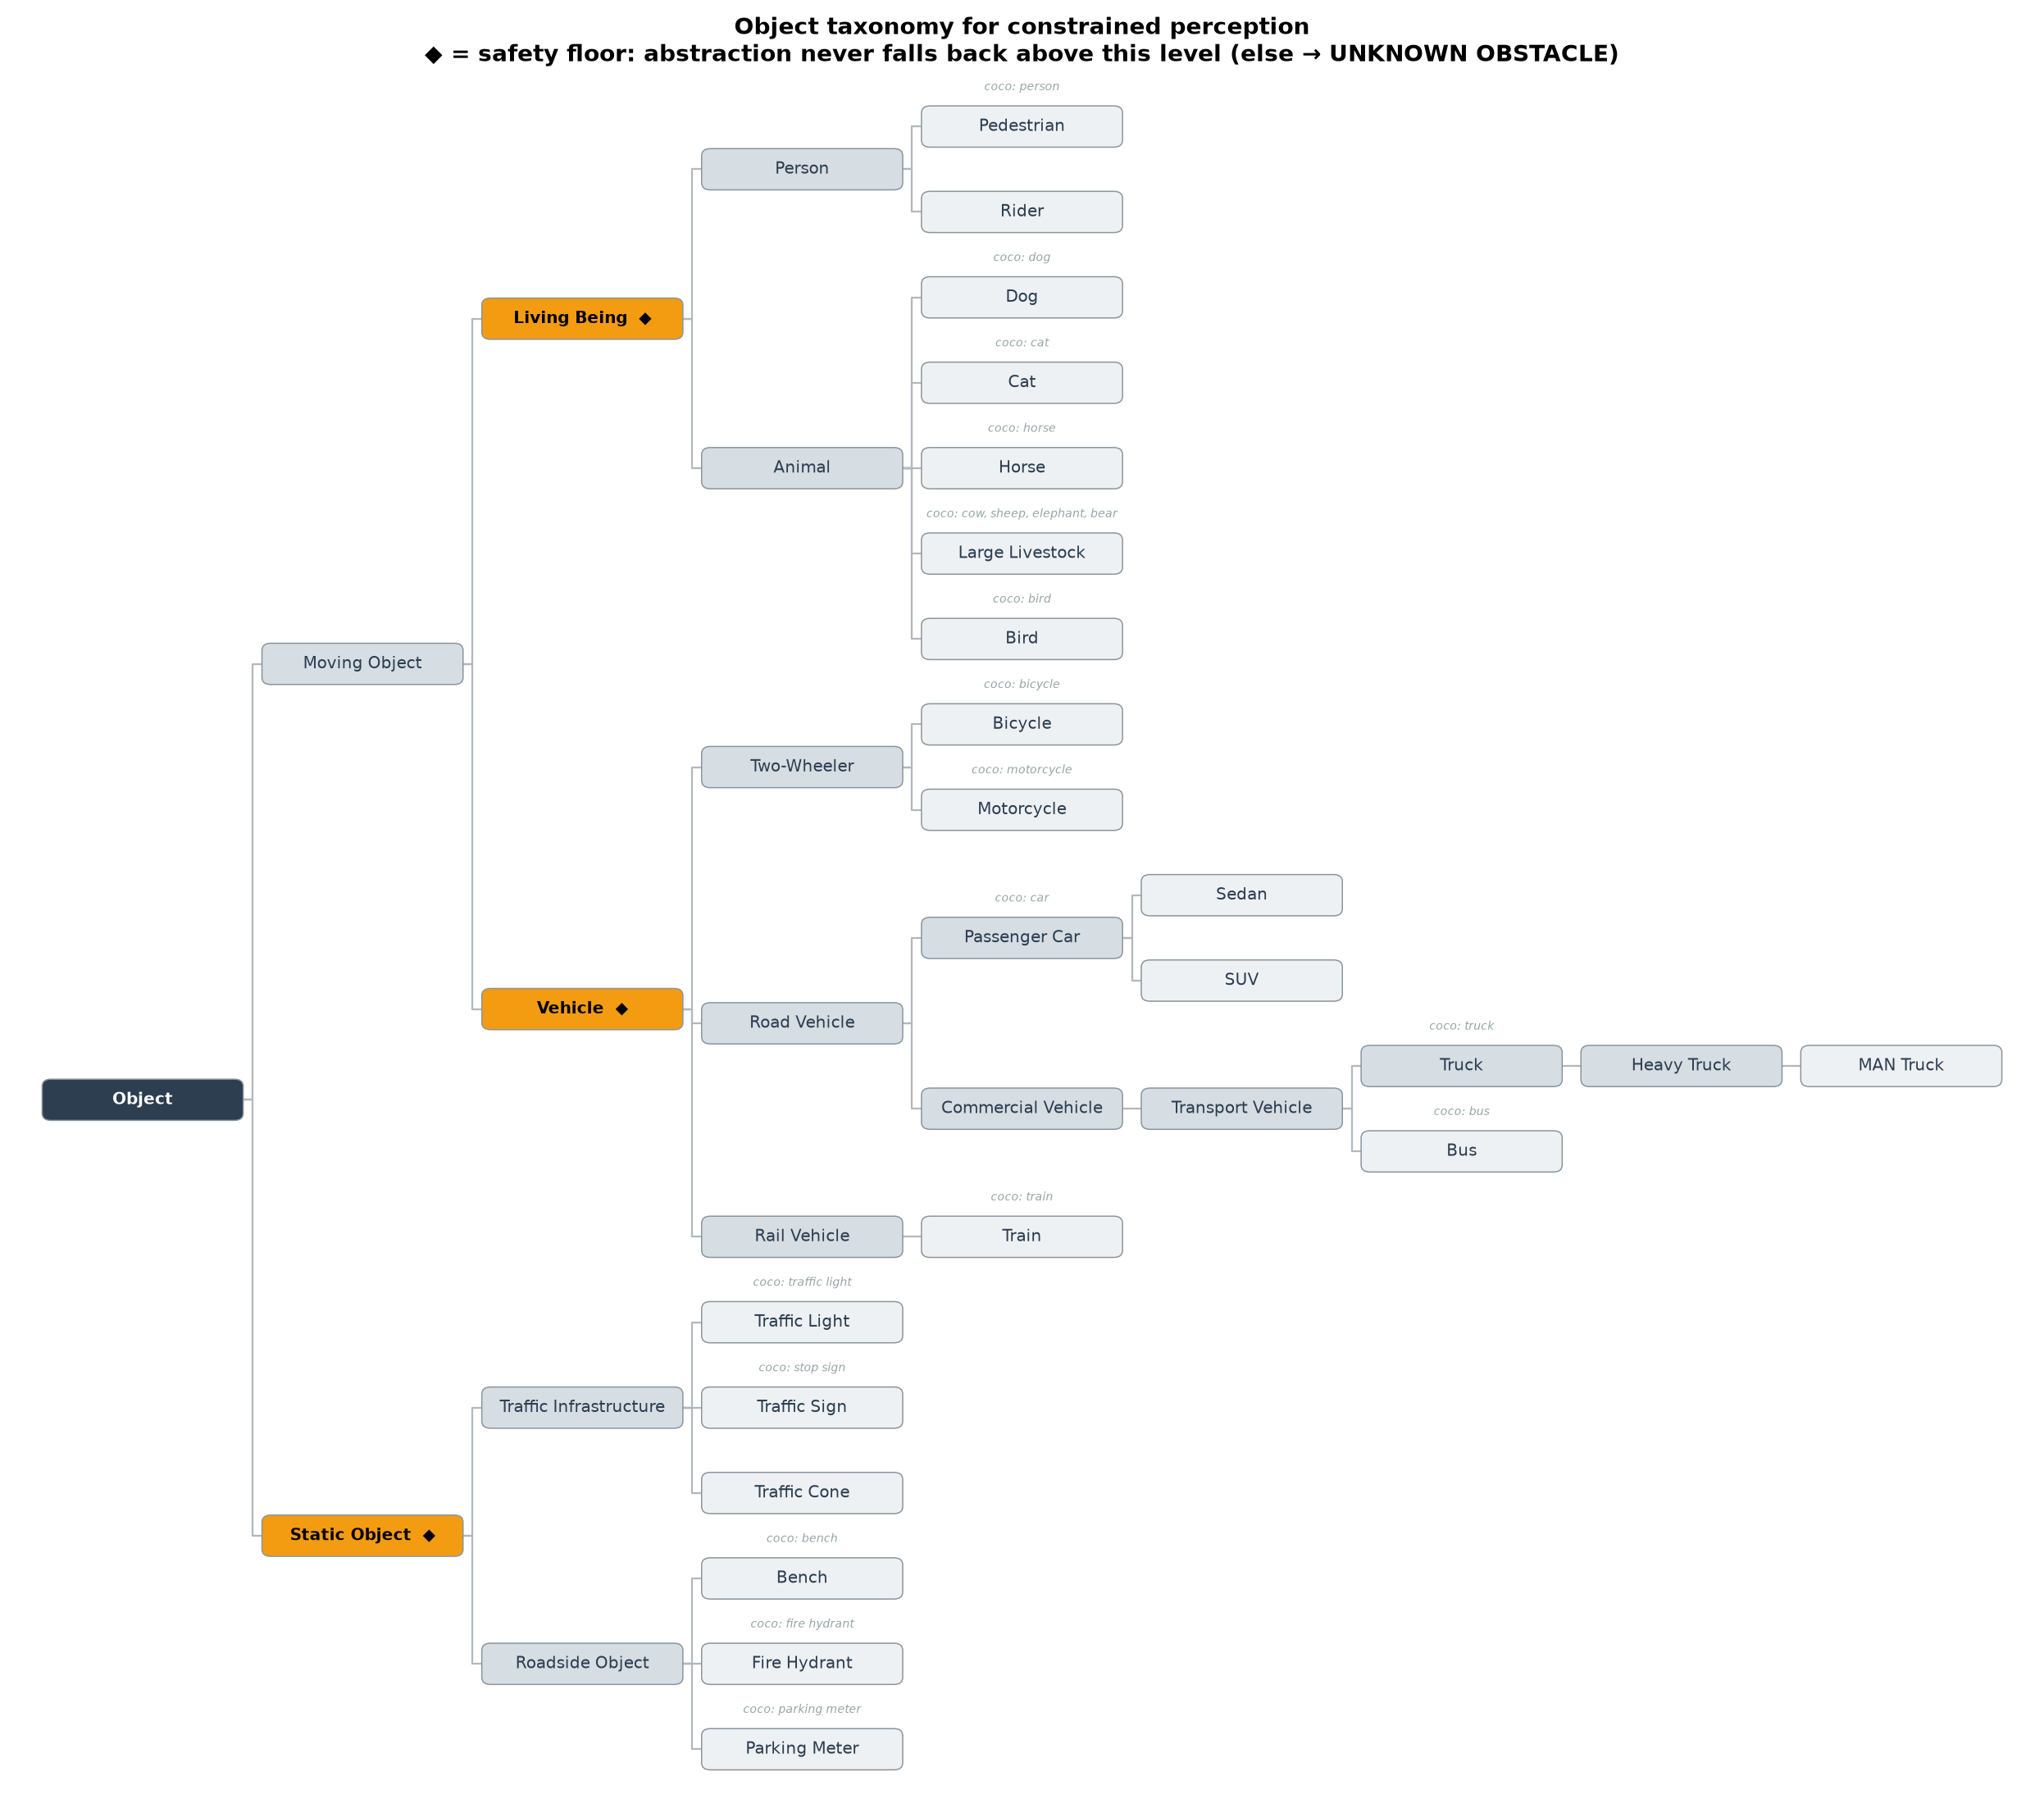
\includegraphics[width=0.96\textwidth]{taxonomy_architecture.png}
\caption{The object taxonomy, rendered from the running configuration. Orange
nodes marked \floor{} are \emph{safety floors}: abstraction may stop at or below
them but never above. Leaves show their detector (COCO) mapping. The deep
\textsf{Truck}$\rightarrow$\textsf{Heavy~Truck}$\rightarrow$\textsf{MAN~Truck}
chain illustrates fine-grained specificity available when evidence supports it.}
\label{fig:taxonomy}
\end{figure*}

\subsection{Detection Front-End and Importance}
Classification cannot help an object that is never boxed, so detection recall is
a prerequisite. A closed-set detector fires only weakly on objects with no
matching class, so we run YOLO~\cite{redmon2016} at \emph{high recall}:
class-agnostic non-maximum suppression and a low confidence threshold, so that
prominent novel objects (an atypical tractor, an overloaded truck) still yield a
box. The taxonomy layer---not the COCO label---then decides the category, and the
constraint gates (Sec.~\ref{sec:method}-D) suppress the extra low-confidence
noise this admits. We emphasize that we do \emph{not} claim an improvement in
detection accuracy here; quantifying that would require bounding-box ground truth
and a detection-metric evaluation, which we leave to future work
(Sec.~\ref{sec:conclusion}).

Not every detection is equally safety-critical: missing a large, near object is
far more dangerous than missing a distant speck. We therefore attach to each
detection an \emph{importance} $\iota = \min(1,\,2\sqrt{a})$, where $a$ is the
box area as a fraction of the frame, and report an importance-weighted version
of the safety metric so that large objects dominate the score.

\subsection{Leaf Scoring}
For each box we take the CLIP~\cite{radford2021} image embedding $\mathbf{z}$ of
the crop and compute its cosine similarity $s_\ell =
\langle\mathbf{z},\mathbf{t}_\ell\rangle$ to the text embedding
$\mathbf{t}_\ell$ of every \emph{leaf} $\ell$. Crucially we score only concrete
leaves, where CLIP is reliable, and never the abstract interior prompts, which
are poorly separated.

\subsection{Mass-Aggregated Abstraction with a Safety Floor}
Leaf similarities are turned into a distribution
$p_\ell = \mathrm{softmax}(s_\ell/\tau)$, and the \emph{mass} of any node $v$ is
the total probability of the leaves in its subtree,
\begin{equation}
m(v) \;=\; \sum_{\ell \in \mathrm{leaves}(v)} p_\ell .
\label{eq:mass}
\end{equation}
Classification is a top-down descent (Alg.~\ref{alg:descent}): starting at the
root, we move into the child holding the largest mass \emph{only while} that mass
exceeds a commit threshold $\theta$; when the mass splits among children the crop
is ambiguous and we stop. The stop node is then checked against the nearest
safety floor: at or below it, the node is reported (a specific leaf $\Rightarrow$
\textsc{identified}; an interior node $\Rightarrow$ \textsc{abstracted}); above
every floor, the detection is reported as \textsc{unknown obstacle}. A global
gate $\sigma_{\min}$ on the best leaf similarity guards against committing to
anything when nothing matches.

\begin{algorithm}[t]
\caption{Hierarchical abstraction with safety floor}
\label{alg:descent}
\begin{algorithmic}[1]
\REQUIRE crop embedding $\mathbf{z}$, taxonomy $T$, thresholds $\theta,\sigma_{\min}$
\STATE $s_\ell \gets \langle\mathbf{z},\mathbf{t}_\ell\rangle$ for all leaves $\ell$;\quad
       $p \gets \mathrm{softmax}(s/\tau)$
\IF{$\max_\ell s_\ell < \sigma_{\min}$}
    \RETURN \textsc{unknown} \COMMENT{nothing matches at all}
\ENDIF
\STATE $v \gets \mathrm{root}(T)$
\WHILE{$v$ has children}
    \STATE $c^\star \gets \arg\max_{c}\, m(c)$ \COMMENT{Eq.~\eqref{eq:mass}}
    \IF{$m(c^\star) \ge \theta$}
        \STATE $v \gets c^\star$
    \ELSE
        \STATE \textbf{break} \COMMENT{mass split $\Rightarrow$ abstract here}
    \ENDIF
\ENDWHILE
\IF{$v$ is at or below a safety floor}
    \RETURN \textsc{identified} if $v$ is a leaf else \textsc{abstracted}
\ELSE
    \RETURN \textsc{unknown obstacle} at $v$
\ENDIF
\end{algorithmic}
\end{algorithm}

\subsection{Context-Constraint Validation}
Finally, each classified detection passes validation gates that reject
physically implausible results: a size range per category (inherited down the
tree) and a position prior that rejects ground objects floating in the sky
region---the classic ``car above the clouds'' false positive~\cite{schaller2025}.
Constraints are cheap, transparent, and independent of the abstraction level.

\section{Experimental Setup}
\label{sec:setup}

\textbf{Data.} We evaluate on the SegmentMeIfYouCan Road~Anomaly
set~\cite{chan2021}, real street scenes containing objects with no proper flat
class (animals, unusual vehicles). Boxes come from YOLOv8s at the high-recall
setting above; CLIP is ViT-B/32. Images are streamed on demand; no training or
fine-tuning is performed at any stage.

\textbf{Novelty oracle.} A detection is \emph{novel} if the detector's COCO class
has no node in our taxonomy (e.g.\ \texttt{giraffe}, \texttt{airplane}); the
correct answer is then a coarse category or an explicit unknown, never a specific
leaf. Otherwise it is \emph{known}, with a ground-truth branch.

\textbf{Fair baseline.} Both systems share the \emph{same} YOLO boxes, the same
CLIP features, and the same leaf vocabulary. The only difference is the decision
rule: the \textsc{flat} baseline takes the arg-max leaf (optionally with a
rejection threshold), and thus can only ever name a specific leaf or drop the
object; the \textsc{hierarchical} system runs Alg.~\ref{alg:descent}. This
isolates the contribution of the hierarchy from detection and representation.

\textbf{Operating point.} A sweep over $(\tau,\theta)$
(Fig.~\ref{fig:calibration}) shows every hierarchical configuration sits at
$100\%$ novel-safety; we select $\tau{=}0.06,\ \theta{=}0.40$, which maximizes
known-object specificity at that safety level.

\section{Results}
\label{sec:results}

Across $40$ images ($54$ detections; $20$ novel, $34$ known),
Table~\ref{tab:results} and Fig.~\ref{fig:benchmark} summarize the comparison.

\begin{table*}[t]
\caption{Flat vs.\ hierarchical, by object population.}
\label{tab:results}
\centering
\begin{tabular}{@{}llccc@{}}
\toprule
Population & Metric & Flat\,(argmax) & Flat\,(reject) & \textbf{Hier.} \\
\midrule
Novel (20) & \textbf{safe-handled}     & $0\%$   & $0\%$   & $\mathbf{100\%}$ \\
Novel      & \ \ importance-weighted   & $0\%$   & $0\%$   & $\mathbf{100\%}$ \\
Novel      & confident wrong leaf      & $100\%$ & $0\%$   & $0\%$   \\
Novel      & dropped (missed)          & $0\%$   & $100\%$ & $0\%$   \\
\midrule
Known (34) & \textbf{useful category}  & $47\%$  & ---     & $\mathbf{77\%}$ \\
Known      & wrong branch              & ---     & ---     & $0\%$   \\
\bottomrule
\end{tabular}
\end{table*}

\subsection{Quantitative}
On \emph{novel} objects the hierarchy handles $100\%$ safely---$9$ abstracted to
a floor category, $11$ flagged \textsc{unknown}---with \emph{zero} confident wrong
leaves. The same $100\%$ holds under \emph{importance weighting}, i.e.\ the large,
safety-critical novel objects are all handled safely. The flat baseline handles
$0\%$ safely by construction: arg-max assigns a wrong leaf to every novel object,
and the rejecting variant instead drops every one, i.e.\ a missed obstacle. The
\emph{safety improvement on novel objects is $+100$ percentage points}.
Importantly, this does not come at the expense of known objects: the hierarchy
gives a useful category to $77\%$ of them (versus $47\%$ for flat arg-max) and
never reports a wrong branch, deferring to an honest \textsc{unknown} on the
remaining $23\%$. Figure~\ref{fig:calibration} shows the result is not a
knife-edge: the hierarchy \emph{dominates} the flat baseline across the entire
operating range.

\begin{figure*}[t]
\centering
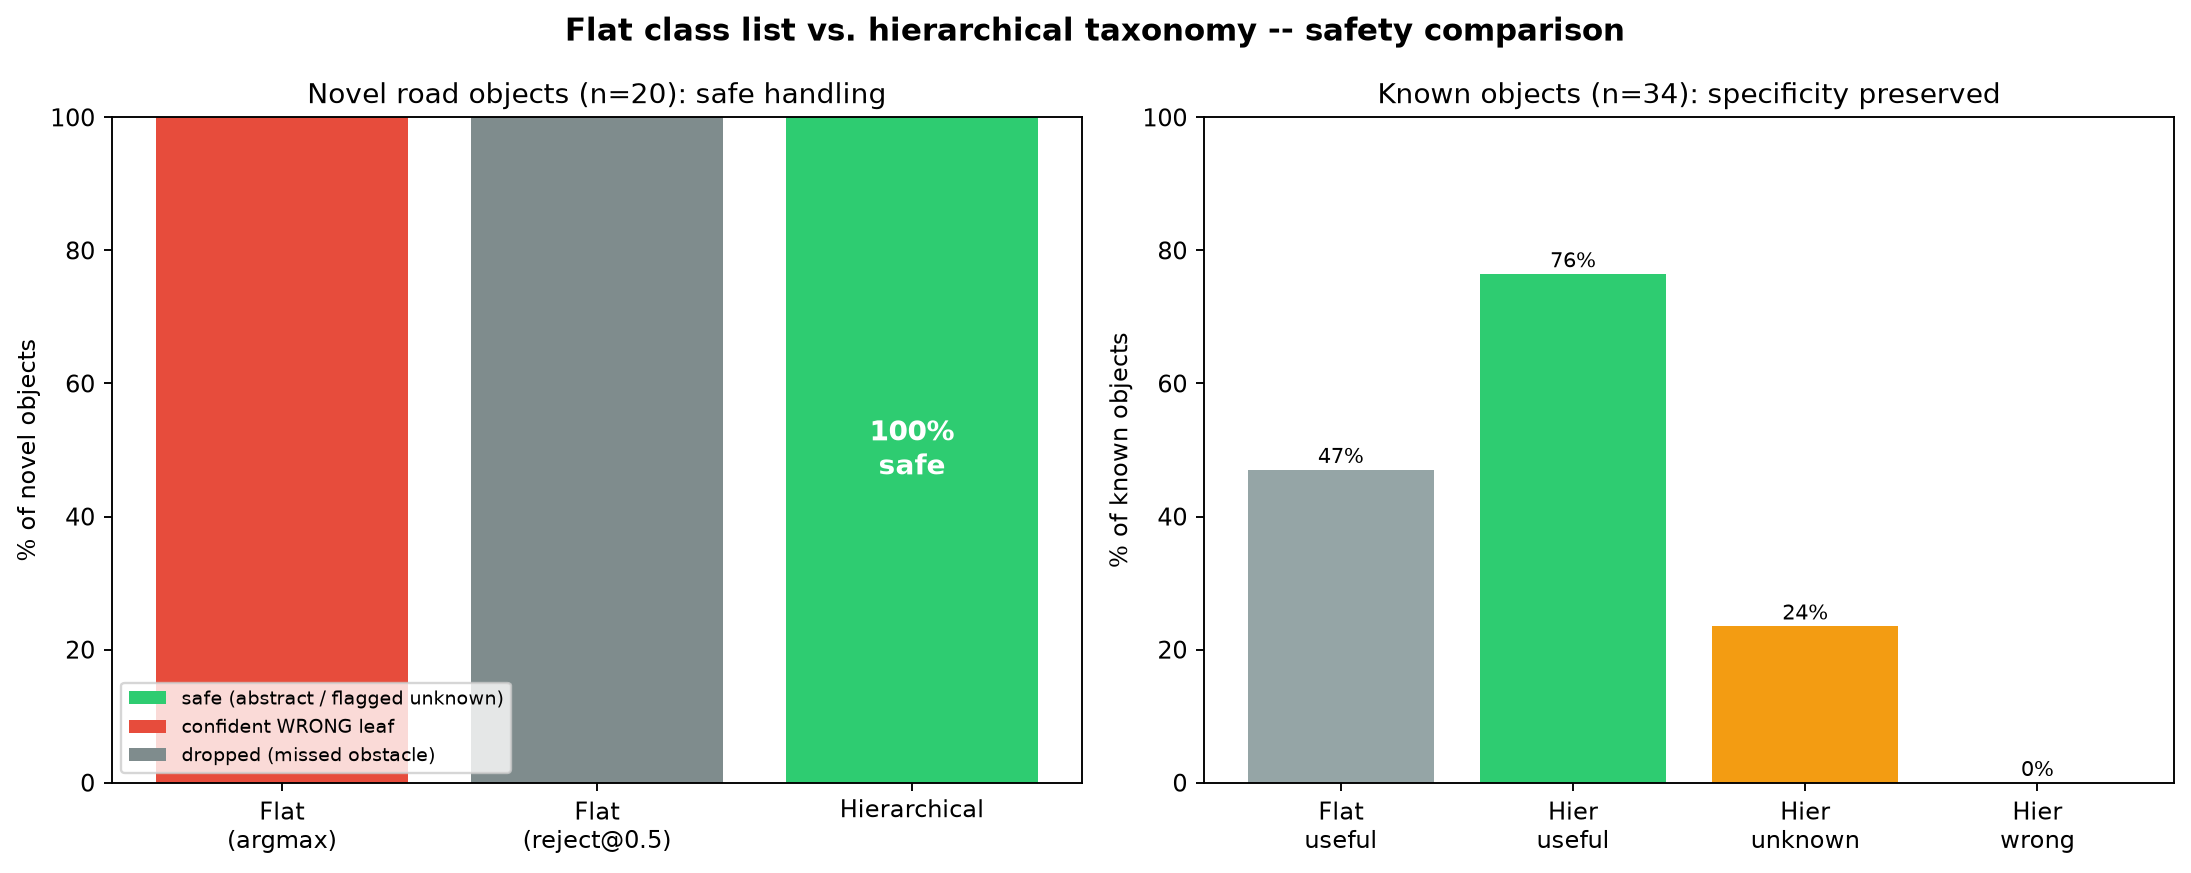
\includegraphics[width=0.96\textwidth]{benchmark_flat_vs_hier.png}
\caption{Left: on novel road objects the hierarchy is $100\%$ safe (abstract or
flagged), while the flat baseline is $0\%$ (a confident wrong leaf, or a dropped
obstacle). Right: on known objects the hierarchy is more specific than flat
arg-max ($77\%$ vs.\ $47\%$ useful) with no wrong-branch claims.}
\label{fig:benchmark}
\end{figure*}

\begin{figure}[t]
\centering
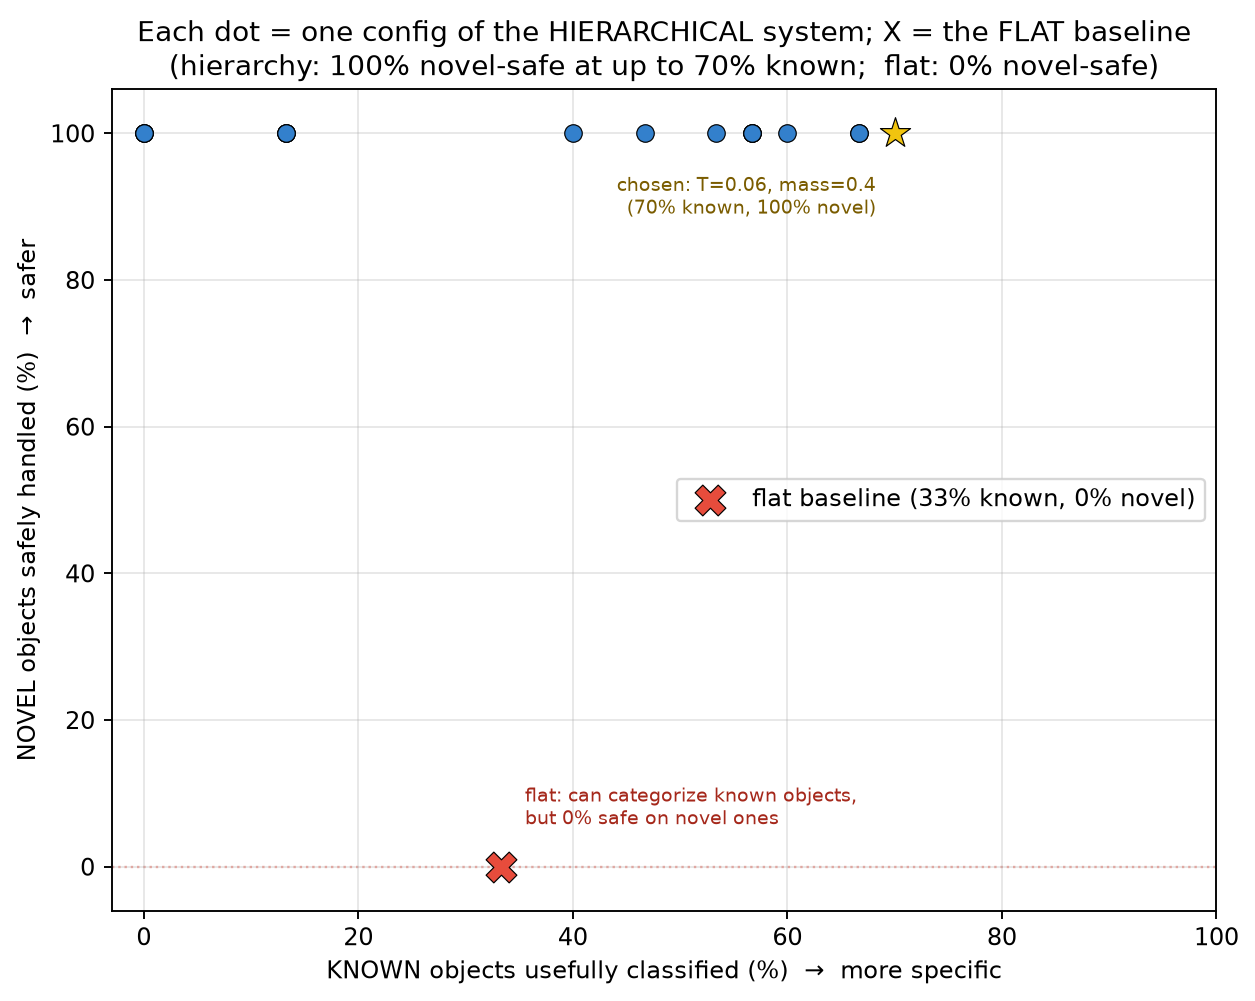
\includegraphics[width=\columnwidth]{calibration_tradeoff.png}
\caption{Operating-point sweep. Each dot is one hierarchical configuration; all
sit at $100\%$ novel-safety while spanning a range of known-object specificity.
The flat baseline (red \textcolor{red}{$\times$}) is a floor at $0\%$
novel-safety. The hierarchy dominates.}
\label{fig:calibration}
\end{figure}

\subsection{Qualitative}
Figure~\ref{fig:giraffe} shows a giraffe on the road. The detector reports
\texttt{giraffe}, which has no taxonomy node; mass concentrates at
\textsf{Moving~Object} and then at \textsf{Living~Being} (a floor), where it
stops---an \emph{abstraction} to a safe, useful category rather than a dropped or
mislabeled obstacle. Figure~\ref{fig:tractor} is the emblematic case: a MAN
tractor towing a covered carriage---a modern analogue of the horse-drawn carriage
of~\cite{schaller2025}, and the largest object in frame (importance $1.0$).
Detected only tentatively (as \texttt{truck}, conf.\ $0.73$), its unusual
articulated form is \emph{not} committed to a specific truck type; the mass
settles at \textsf{Vehicle}---exactly the ``shared moving-vehicle category'' the
original argument calls for. Of the $20$ novel objects, the $11$ that are
genuinely cross-categorical instead bottom out as \textsc{unknown obstacle} above
the floor---the deeper safety net.

\begin{figure}[t]
\centering
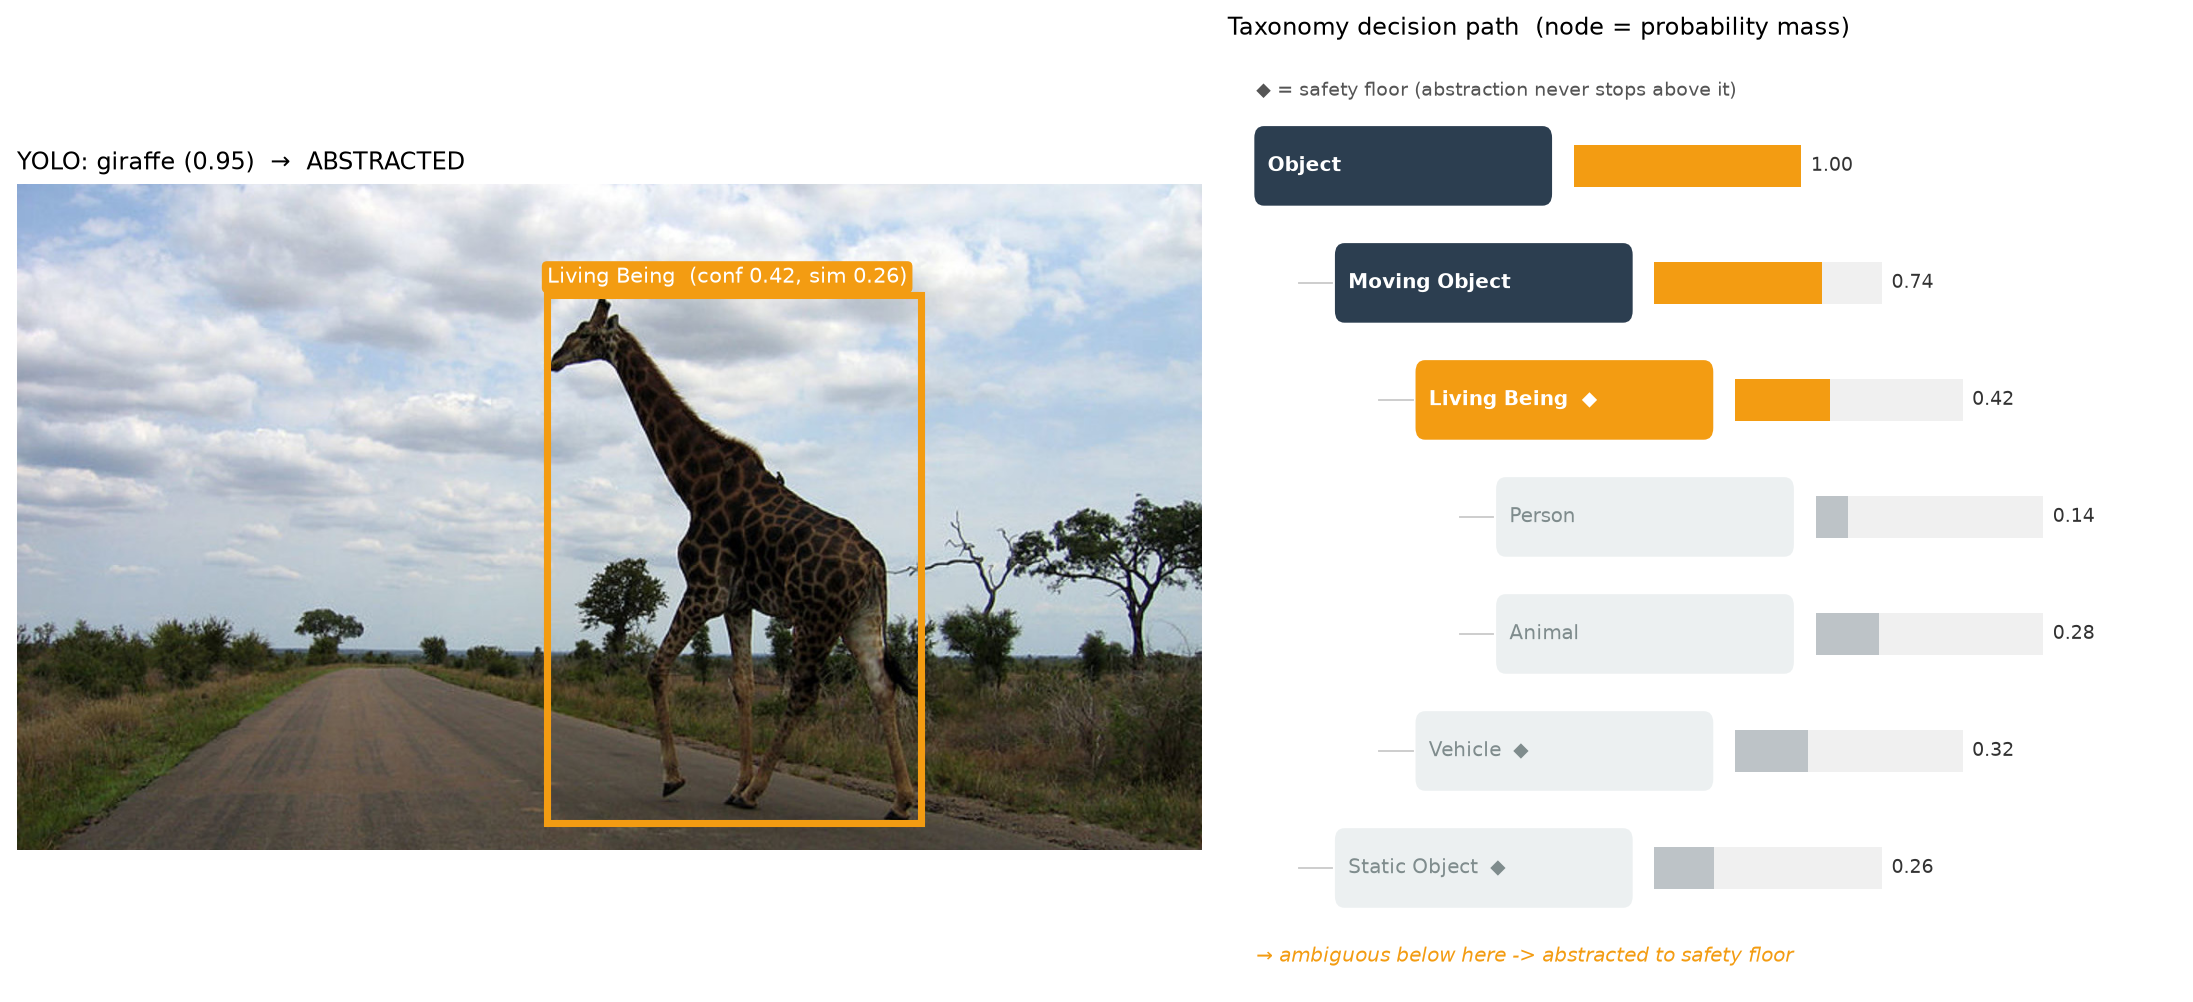
\includegraphics[width=\columnwidth]{ex_road_anomaly_01_0_abstracted.png}
\caption{\textsc{Abstracted}. A giraffe (no taxonomy leaf) is not dropped: the
mass climbs to \textsf{Living~Being}, a safety floor, and stops. Top: the
detection (with confidence, CLIP similarity, and importance); bottom: the
per-node probability mass along the decision path.}
\label{fig:giraffe}
\end{figure}

\begin{figure}[t]
\centering
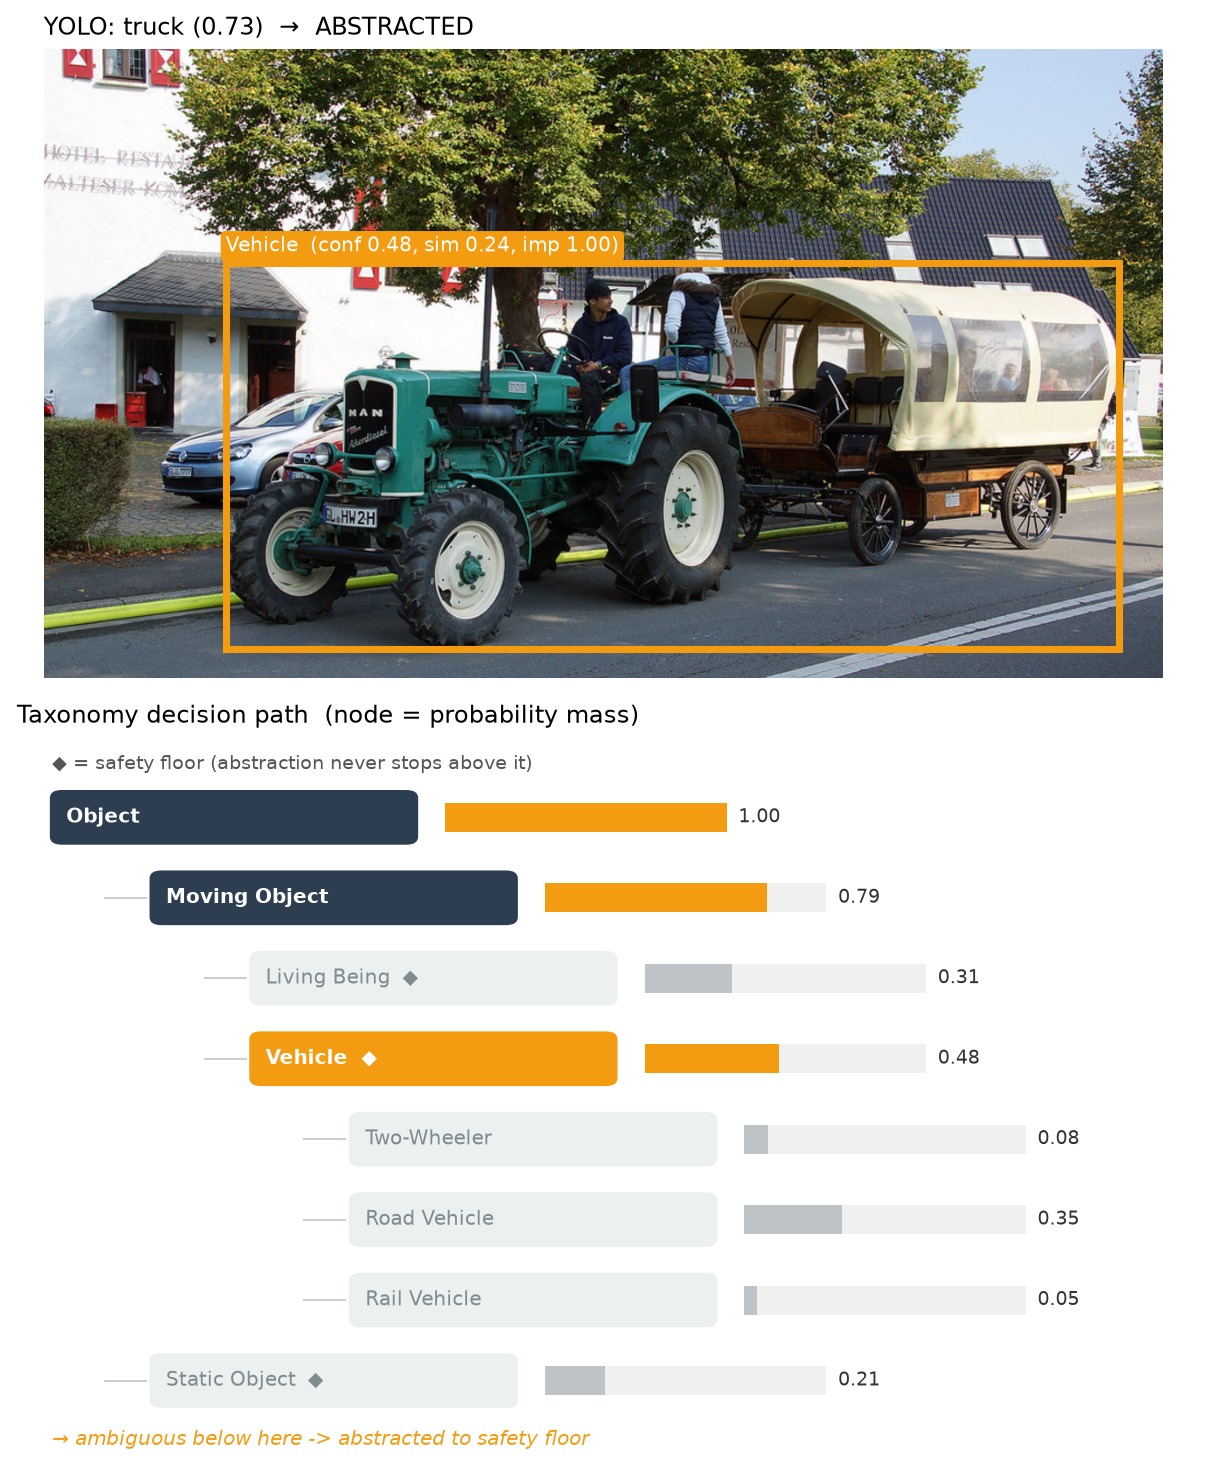
\includegraphics[width=\columnwidth]{ex_road_anomaly_08_1_abstracted.png}
\caption{\textsc{Abstracted}, emblematic. A MAN tractor towing a covered carriage
---detected only tentatively as \texttt{truck}---is safely classified as
\textsf{Vehicle} rather than a wrong specific type. It is the largest, most
important object in frame (importance $1.0$); missing or mislabeling it would be
the worst failure.}
\label{fig:tractor}
\end{figure}

\section{Discussion}
\label{sec:discussion}

The results expose a subtlety worth stating plainly. Our system does \emph{not}
label every unusual object \textsc{unknown}; it labels it as specifically as the
evidence safely allows. A visibly overloaded but clearly wheeled vehicle
abstracts to \textsf{Vehicle}; only genuinely cross-categorical cases become
\textsc{unknown}. This graded behavior is the intended one: maximal specificity
subject to a safety floor. It is also the epistemically honest response to the
\emph{scale-dependent decidability} of~\cite{schaller_patterns}: a distant or
ambiguous object supports a specific hypothesis only at a resolution the sensor
may not have, so abstracting---rather than hallucinating a confident leaf---is the
system calculating its own semantic ignorance rather than denying it.

\textbf{Limitations.} The novelty oracle is derived from the detector's own class
vocabulary rather than pixel-level ground truth, and the study is at the scale of
tens of images on one anomaly set. The ``identified-to-a-leaf'' rate on known
objects is $0\%$ because several COCO classes map onto \emph{interior} taxonomy
nodes (e.g.\ \texttt{car}$\rightarrow$\textsf{Passenger~Car}, whose Sedan/SUV
leaves split the mass); ``useful category on the correct branch'' is therefore
the meaningful specificity measure. The high-recall detection setting also admits
false positives, which the constraint gates mitigate but do not eliminate; and
because we lack box ground truth, missed (large) objects cannot be measured here,
so our importance weighting scores only \emph{detected} objects. Finally, CLIP on
small crops is the accuracy bottleneck, not the abstraction logic.

\section{Conclusion and Future Work}
\label{sec:conclusion}

Replacing the flat class list with a hierarchical taxonomy and a mass-aggregated
abstraction rule, bounded by a safety floor, converts the open-world failure mode
of driving perception---mislabel-or-drop---into a safe, graded fallback:
$+100$ percentage points of safe handling on novel objects at no cost to known
ones. The mechanism is training-free and rides on off-the-shelf detection and
open-vocabulary models.

Three directions follow. \emph{First, and most fundamental: train the detector
itself on the taxonomy, not on a flat class list.} A closed-set detector
struggles with the tractor not because the object is invisible but because its
label space has no slot for ``some kind of moving vehicle.'' Re-training the
detector to predict \emph{hierarchical} targets---so that an object it cannot
resolve to a leaf may be emitted at an abstract node---would raise recall on
exactly the novel objects this work targets. Crucially this must be a
\emph{taxonomic}, not a flat, extension: appending an abstract label
(``vehicle'') as one more entry in a list of specific classes (``sedan, truck,
bus'') is a category error---mixing levels of abstraction in one flat list is
both semantically meaningless and a source of confusion for the model---whereas a
hierarchy places the abstract node \emph{above} the specific ones, where it
belongs. We do not know precisely what the tractor is; we only know it behaves
like a moving vehicle, and a hierarchically-trained detector could say exactly
that. \emph{Second}, on a box-annotated corner-case set (e.g.\ CODA~\cite{li2022}
or BDD100K), evaluate the front-end with proper detection metrics (recall,
precision, mAP), importance-weighted, to test whether semantic filtering of
high-recall proposals measurably improves \emph{usable} detection of novel
objects---a claim we deliberately do not assert here without that evidence.
\emph{Third} (v2), add a second, independent perception path: \emph{semantic
segmentation} as a parallel taxonomy and cross-validation layer. Beyond rejecting
implausible detections (a ``vehicle'' whose region segments as sky), segmentation
supplies \emph{additional scene-context labels}---drivable lane, sidewalk,
parking strip---that feed back into the taxonomy decision itself. Knowing that an
object sits on the active carriageway rather than parked at the roadside is direct
evidence for the \textsf{Moving~Object} versus \textsf{Static~Object} split at the
top of the tree; a segmentation cue that the region is a moving road user thus
sharpens exactly the coarse distinction the safety floor depends on. In other
words, the second modality does not merely validate the first---it enriches the
taxonomic evidence and can raise the level at which the system can safely commit.

\emph{Fourth}, and as the culmination, add \emph{3D scene reconstruction}.
Monocular reconstruction already recovers static structure, but its blind spot is
precisely motion. The decisive step is \emph{stereo}: synchronous capture
separates space from time, so that ego-motion (the whole scene sweeping past as
parallax) can be factored out and any object whose displacement deviates from that
parallax field is revealed as independently moving. Extracting such motion vectors
makes dynamic objects pop out of the static background and provides direct,
geometric evidence for the \textsf{Moving~Object} branch---the very split the
safety floor rests on. This distinction is not academic: static objects need only
be driven around, whereas a moving object may enter the ego-vehicle's trajectory,
so it demands the most attention and, ultimately, \emph{prediction}---estimating
its future from its present and past. A taxonomy that fuses appearance (CLIP),
context (segmentation), and motion (stereo) could commit to \textsf{Moving
Object} on geometry alone even when appearance is ambiguous, closing the loop from
detection to safe, forward-looking behavior.

Together these move the system toward the multi-level semantic validation argued
for in~\cite{schaller2025}.

\newpage
\begin{thebibliography}{9}
\bibitem{schaller2025}
F.~Schaller, ``The Role of Semantic Models in Constraining Pattern Recognition in
Modern AI Systems,'' in \emph{Intelligent Environments 2025: Combined Workshop
Proc.}, IOS Press, 2025, pp.~96--105, doi:10.3233/AISE250023.

\bibitem{schaller_patterns}
F.~Schaller, ``Patterns Everywhere, Context Nowhere: Decidability and the
Semantic Crisis in Autonomous Systems,'' Zenodo, 2026. % TODO: add Zenodo DOI

\bibitem{radford2021}
A.~Radford et al., ``Learning Transferable Visual Models From Natural Language
Supervision,'' in \emph{Proc. ICML}, 2021.

\bibitem{redmon2016}
J.~Redmon, S.~Divvala, R.~Girshick, and A.~Farhadi, ``You Only Look Once:
Unified, Real-Time Object Detection,'' in \emph{Proc. IEEE CVPR}, 2016,
pp.~779--788.

\bibitem{bertinetto2020}
L.~Bertinetto, R.~Mueller, K.~Tertikas, S.~Samangooei, and N.~Lord, ``Making
Better Mistakes: Leveraging Class Hierarchies with Deep Networks,'' in
\emph{Proc. IEEE CVPR}, 2020, pp.~12506--12515.

\bibitem{chan2021}
R.~Chan et al., ``SegmentMeIfYouCan: A Benchmark for Anomaly Segmentation,'' in
\emph{Proc. NeurIPS Datasets and Benchmarks}, 2021.

\bibitem{li2022}
K.~Li et al., ``CODA: A Real-World Road Corner Case Dataset for Object Detection
in Autonomous Driving,'' in \emph{Proc. ECCV}, 2022, pp.~406--423.

\bibitem{sedeh2021}
A.~Rausch, A.~M.~Sedeh, and M.~Zhang, ``Autoencoder-based Semantic Novelty
Detection: Towards Dependable AI-based Systems,'' \emph{Applied Sciences},
vol.~11, no.~21, p.~9881, 2021.

\bibitem{bender2021}
E.~M.~Bender, T.~Gebru, A.~McMillan-Major, and S.~Shmitchell, ``On the Dangers of
Stochastic Parrots: Can Language Models Be Too Big?,'' in \emph{Proc. ACM FAccT},
2021, pp.~610--623.

\bibitem{rosch1975}
E.~Rosch, ``Cognitive Representations of Semantic Categories,'' \emph{J.\ of
Experimental Psychology: General}, vol.~104, no.~3, p.~192, 1975.
\end{thebibliography}

\end{document}
